\subsection{Frequency Noise}
In this section image 4.1 is considered.
As the image contains a lot of disturbance in form of lines, a frequency analysis of the image was made.
The magnitude plot of a cutout of the uniform area of image 4.1 is seen in figure \ref{fig:freq_analysis_uni_p4} and the magnitude plot for the whole image in \ref{fig:freq_analysis_p4}.



\begin{figure}[H]
\centering
\begin{tikzpicture}
\node {\includegraphics[width = 0.9 \linewidth]{../code/images/frequency_analysis_uni_04.png}};

\node[circle, draw, minimum width = 0.3cm,red,very thick] at (1.45, 1.41) {};

\node[circle, draw, minimum width = 0.3cm,red,very thick] at (-1.30, -1.42) {};

\node[circle, draw, minimum width = 0.3cm,blue,very thick] at (-0.39, 0.46) {};

\node[circle, draw, minimum width = 0.3cm,blue,very thick] at (0.54, -0.48) {};
\end{tikzpicture}
\caption{Magnitude plot of the uniform area of image 4.1 in the frequency domain.}
\label{fig:freq_analysis_uni_p4}
\end{figure}


\begin{figure}[H]
\centering
\begin{tikzpicture}

\node {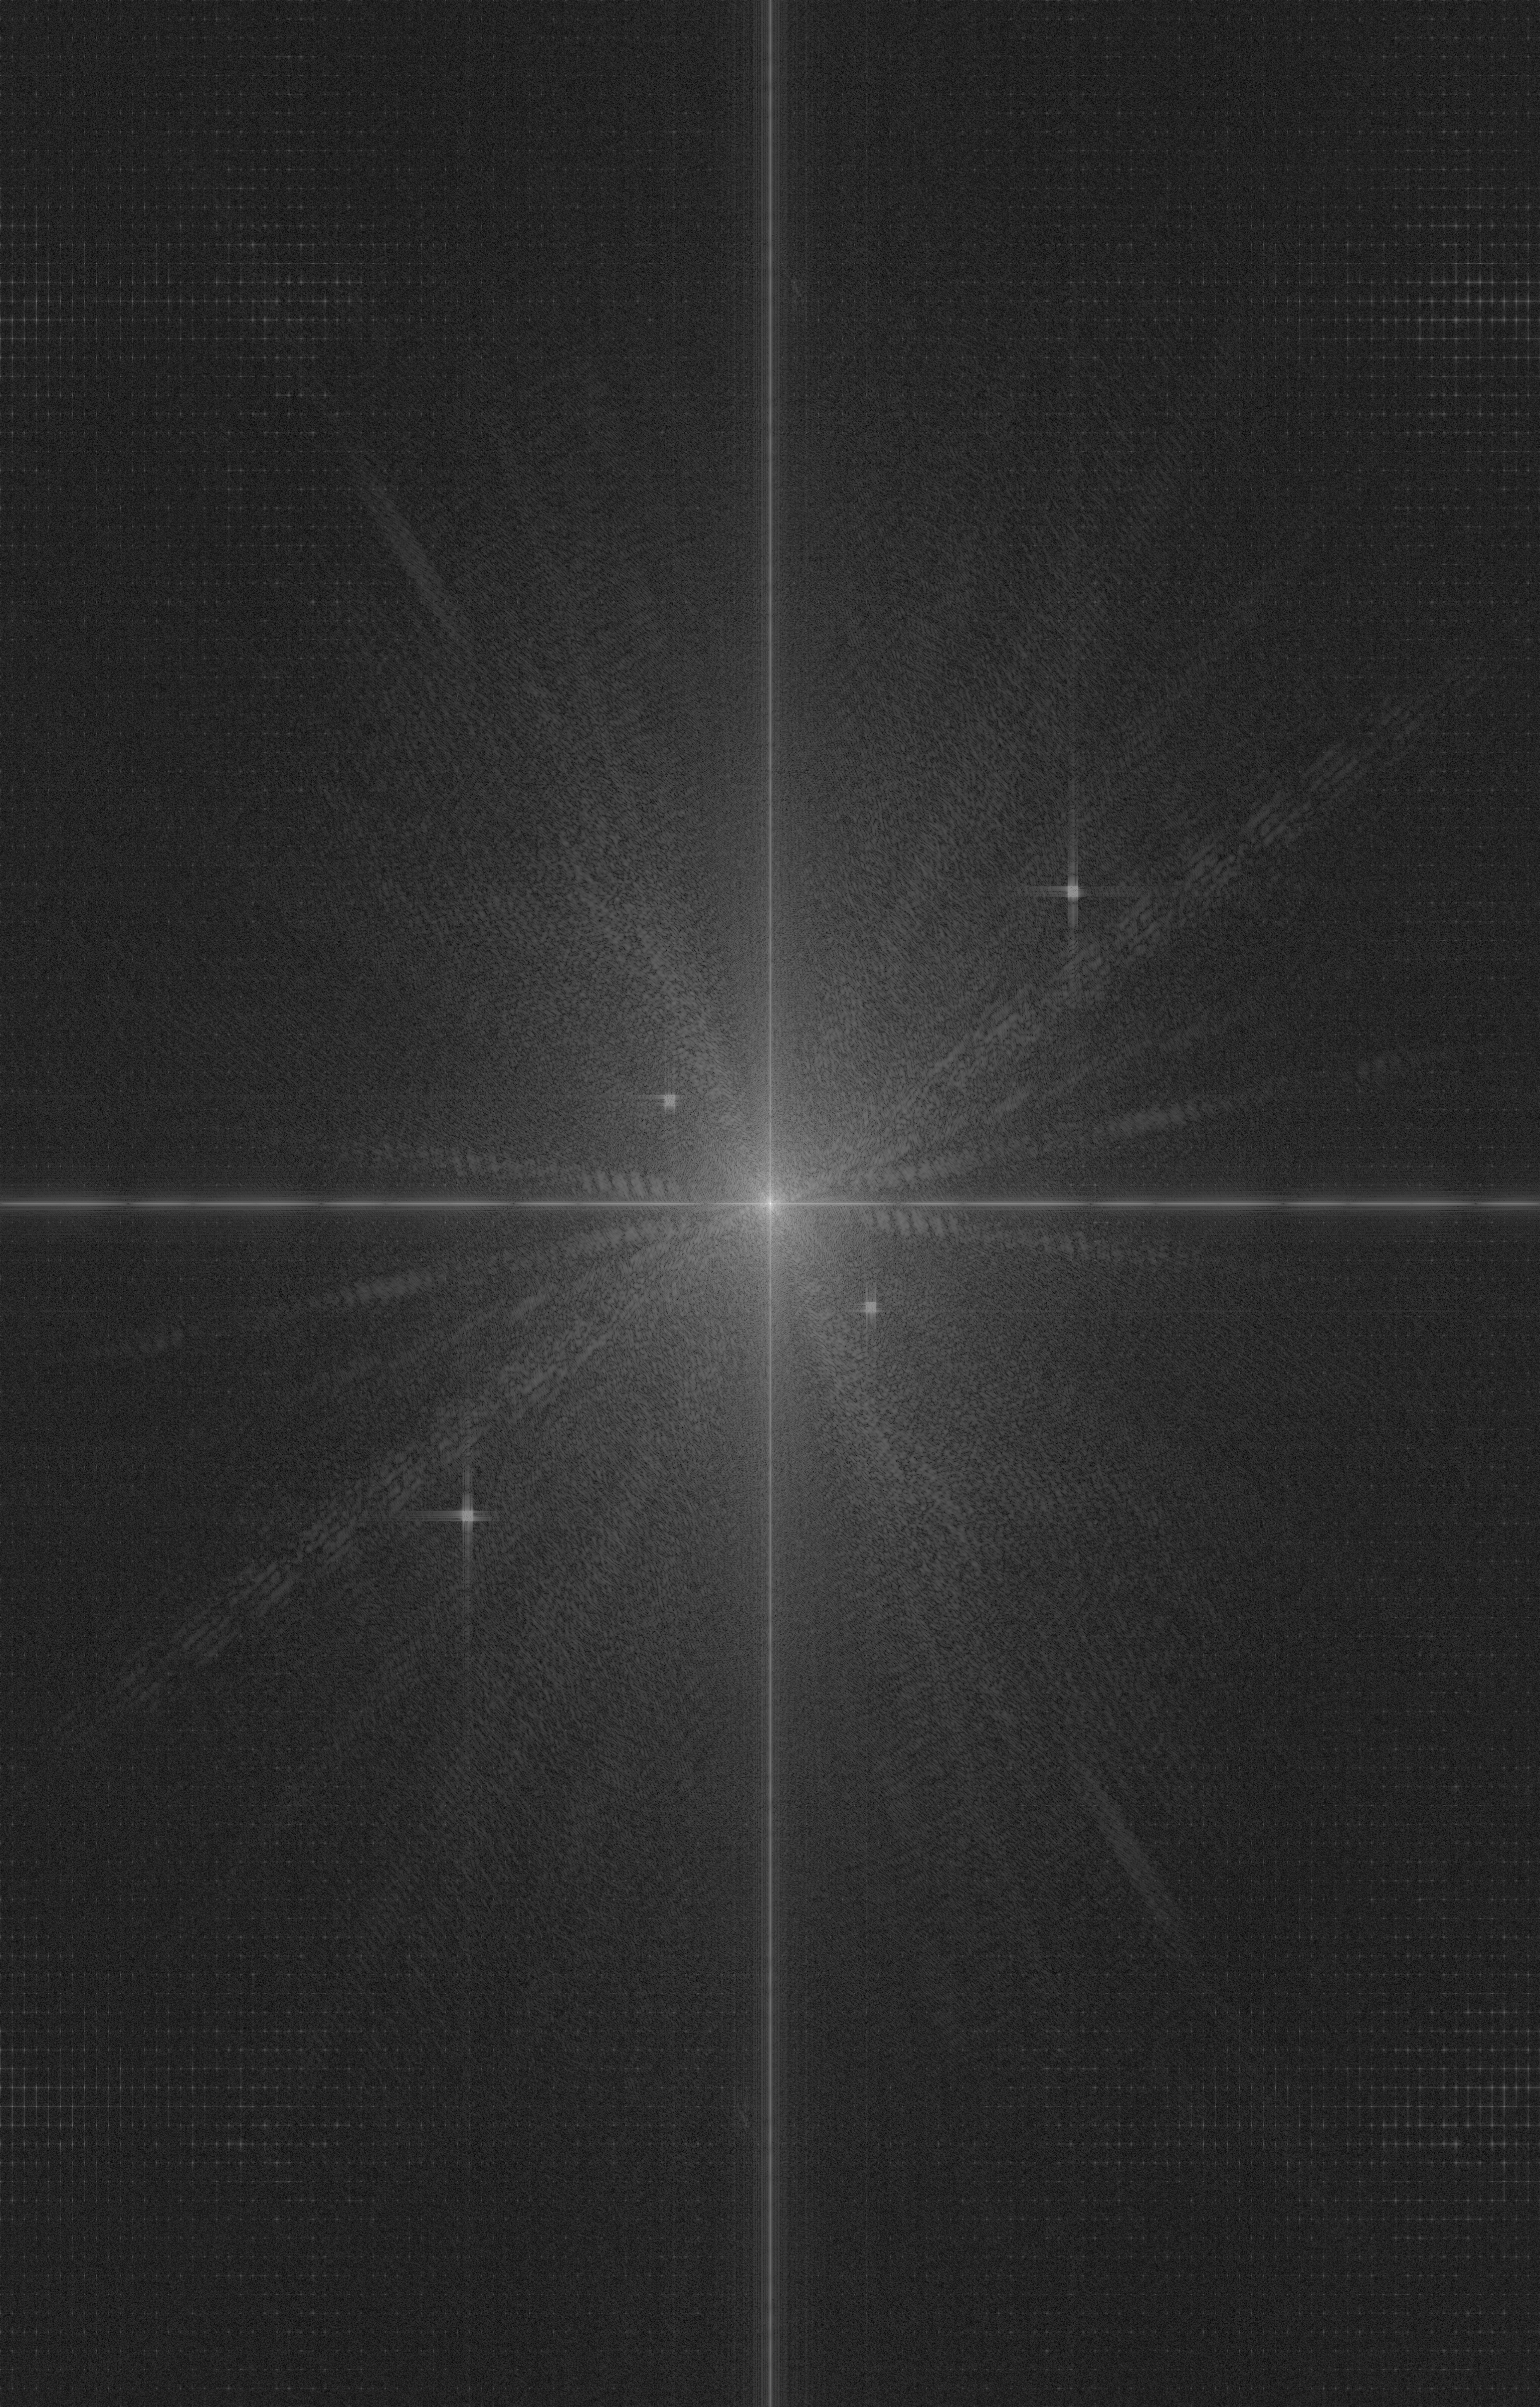
\includegraphics[width = 0.9 \linewidth]{../code/images/frequency_analysis_04.png}};

\node[circle, draw, minimum width = 0.3cm,red,very thick] at (1.45, 1.41) {};

\node[circle, draw, minimum width = 0.3cm,red,very thick] at (-1.30, -1.42) {};

\node[circle, draw, minimum width = 0.3cm,blue,very thick] at (-0.39, 0.46) {};

\node[circle, draw, minimum width = 0.3cm,blue,very thick] at (0.54, -0.48) {};
\end{tikzpicture}

\caption{Magnitude plot of image 4.1 in the frequency domain.}
\label{fig:freq_analysis_p4}
\end{figure}


Figure \ref{fig:freq_analysis_uni_p4} is the frequency analysis of the uniform area of image 4.1.
This should ideally only contain the DC component when no noise is present.
It can therefore be concluded the the bright spots present on figure \ref{fig:freq_analysis_uni_p4}, apart from the DC component, must be caused by the disturbance.
These point pairs are circled on figure \ref{fig:freq_analysis_uni_p4} with each pair their own color.
The two disturbances originate from the lines at an approximate $\pm 45$ degrees angle from the horizon.

These points of disturbance can then be mapped directly onto the magnitude plot of the whole image.
In figure \ref{fig:freq_analysis_p4} the disturbance pairs are marked in the same color as on figure  \ref{fig:freq_analysis_uni_p4}.


In order to remove the disturbances, it was chosen to use a Butterworth filter located at the origin of the disturbances.
The cut-off frequency was chosen to be the distance from the center of the disturbance to its furthest clearly visible edge.

When the filters were applied to the image and the images then turned back into the spacial domain, figure \ref{fig:result_04} was the result of the filtering.


\begin{figure}[H]
\centering
\includegraphics[width = 0.9 \linewidth]{../code/images/image_result_04.png}
\caption{Resulting image after filtering the disturbance from image 4.1 in the frequency domain.}
\label{fig:result_04}
\end{figure}
